WebGL can be referred to as one of the easiest 3D API to use.
In contrast to other APIs one does not have to worry about makefiles, includes, linking the libraries etc. 
WebGL applications consist of control code written in JavaScript and special effects code (shader code) that is executed on a computer's Graphics Processing Unit (GPU).
The first thing one will need in order to use WebGL to render in 3D is to retrieve from the DOM (or create dynamically) the Canvas element and to get a context as shown in Listing~\vref{lst:webgl_create_canvas}.

\begin{filecode}[language=JavaScript,label=lst:webgl_create_canvas,
caption=Create Canvas element and get the context for rendering with WebGL.]
  \lstinputlisting{./code/webgl_create_canvas.js}
\end{filecode}

After using the code in Listing~\ref{lst:webgl_create_canvas} one can observe in current webpage's DOM the canvas element (if it hasn't been created before) that can be used for WebGL rendering.
Normally one would define other parameters after getting WebGL context, e.g.:

\begin{itemize}[leftmargin=0.4cm]
\item \texttt{gl.clearColor(0.0, 0.0, 0.0, 1.0)} - set context's clearing color (black was used in here),
\item \texttt{gl.enable(gl.DEPTH\_TEST)} - enable depth testing,
\item \texttt{gl.depthFunc(gl.LEQUAL)} - set depth function so that near objects hide the further placed objects,
\item \texttt{gl.clear(gl.COLOR\_BUFFER\_BIT|gl.DEPTH\_BUFFER\_BIT)} - \newline clear the color (to the value set with \texttt{clearColor}) as well as the depth buffer (set with \texttt{depthFunc}).
\end{itemize} 

WebGL manages a rectangular viewport (almost the same as in OpenGL since it was derived from it) as part of its state which defines the placement of the rendering results in the drawing buffer.
It can be referred to as the area of one's canvas that the rendering will be drawn and it is responsible for translating model's coordinates to view's and finally viewport's coordinates.
A newly created WebGL context will set its viewport resolution equal to the height and width of its canvas element, without any scripting, HTML or CSS, at the instant the context was obtained.
\newline Editing the style of a canvas element (e.g. width and height) will change its displayed size but will not change its rendering resolution.
Editing those attributes of canvas element after the context has been created will also not change the number of pixels to be drawn.
\newline To change the resolution which WebGL renders at, such as when the user resizes the window or the resolution change in adjustable graphics settings, one will need to call WebGL context's \texttt{viewport()} function to acknowledge the change.
Changing the viewport for WebGL is as simple as calling \texttt{gl.viewport(x, y, width, height)}; with (x,y) being the positions of the viewport and (width, height) the size of the viewport. 
Most of the time those variables describing new size of the viewport will match the dimensions of one's canvas, but there are some scenarios where one would only want to draw a part of it (for instance split-screen gaming).

To decide what and how will be lit on the scene that one try to render with WebGL and what colors it will take, one have to provide two shaders\footnote{In computer graphics, short program written in a shader language that describes properties of pixels and vertices on the redered context.} to instruct WebGL context about colors and positions.
\newline Shaders are specified using the OpenGL ES Shading Language\cite{glsl_es_manpages} (GLSL ES).
Shaders supplied to WebGL context consist of:
\clearpage

\begin{itemize}
\item Vertex shader which processes every vertex that has been passed to WebGL (OpenGL) context, transforming the positions into clipspace coordinates and setting up any values that should be interpolated across connected vertices such as colors or texture coordinates, here context will use normals to compute a lighting factor based on the normals of each triangle.
In vertex shader code one can define the following: 
\begin{itemize}
\item Vertex position transformation using the modelview and projection matrices,
\item Normal transformation, and if required its normalization,
\item Texture coordinate generation and transformation,
\item Lighting per vertex or computing values for lighting per pixel,
\item Color computation.
\end{itemize}
\item Fragment shader is a unit that is reponsible for calculating the colors of every pixel in the context. Pixel shading is most often used for providing shadows on the scene or similar effects, e.g.: bump-mapping.
This unit is responsible for operations, e.g.:
\begin{itemize}
\item Computing colors and texture coordinates per pixel,
\item Computing normals, if you want lighting per pixel,
\item Texture application,
\item Fog computation.
\end{itemize}
\end{itemize}

\begin{wrapfigure}{r}{0.6\textwidth}
%\begin{figure}[h!]
	\vspace*{-0.65in}
	\hspace*{1em}
	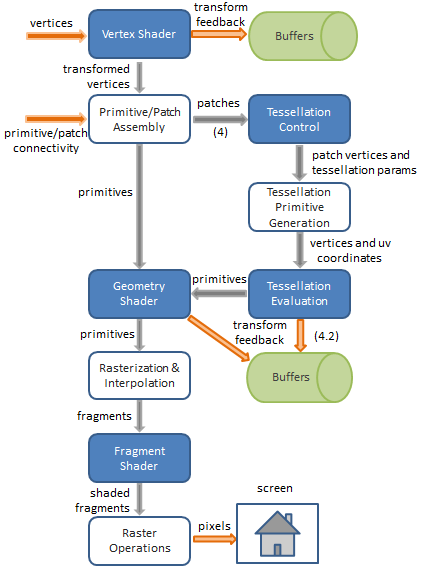
\includegraphics[height=0.47\textheight,keepaspectratio]{webgl_pipeline.png}
	\caption{WebGL's pipeline diagram~\cite{lighthouse3d_pipeline}}
	\label{fig:webgl_pipeline}
%\end{figure}
\end{wrapfigure}
\vspace{1pc}

Yet, it may seem that they are slightly similar they operate on totally different objects.
\newline Vertex shader operates only on each vertex individually not having a clue about remaining vertices.
\newline Fragment shader on the other hand operates on fragments\footnote{Data necessary to generate single pixel's worth of a drawing primitive in the frame buffer, e.g.: raster position, depth, interpolated attributes (color, texture coordinates, etc.), alpha value.}.
One can say that fragment shader takes care how pixels look in between the vertices (they interpolate the pixels' values following special rules defined in fragment shader).
Figure~\ref{fig:webgl_pipeline} shows WebGL's pipeline with vertex and fragment shaders marked there.

\clearpage

Vertex and fragment shaders have acces to OpenGL state, therefore they have access to state matrices like:
\begin{itemize}
\item Projection matrix (\texttt{uniform mat4 gl\_ProjectionMatrix}) - converts eye coordinates to clip coordinates,
\item Modelview matrix (\texttt{uniform mat4 gl\_ModelViewMatrix}) - result of multiplication of two matrices: 
\begin{itemize}
\item Model matrix which transforms object from object coordinates to world coordinates,
\item View matrix which converts world coordinates to eye coordinates. 
\end{itemize}
\end{itemize}

To completely be able to manipulate the vertex data one will need the incoming vertex that is fed to vertex shader.
This can be accessed by \texttt{attribute vec4 gl\_Vertex}
With those variables' (and many others fully listed in WebGL specification) one can manipulate the vertex data in vertex shader.
Fragment shader also has access to OpenGL state so using for instance \texttt{gl\_FragColor} it can set output fragment color.
Exemplar code of shaders is shown in Listing~\ref{lst:webgl_simple_shaders}. 

\begin{filecode}[label=lst:webgl_simple_shaders,language=HTML,caption=Exemplar implementation of vertex and fragment shaders written in GLSL ES.]
\lstinputlisting{./code/webgl_simple_shaders.html}
\end{filecode}